\section{Address Decoding}
\begin{itemize}
  \item Decoding address sent from $\mu P$ is necessary, as without it, only one memory device can be connected to a $\mu P$
  \item Another reason of decoding is possible mismatch (or difference) between the numbr of connections in $\mu P$ and memory.

\end{itemize}
\textbf{Example}: a 2K x 8 EPROM (2716) has 11 address pins, whereas the $\mu P$ 8088 has 20 address pins.
\subsection{Simple NAND Gate Decoder}

\begin{figure}[h!]
  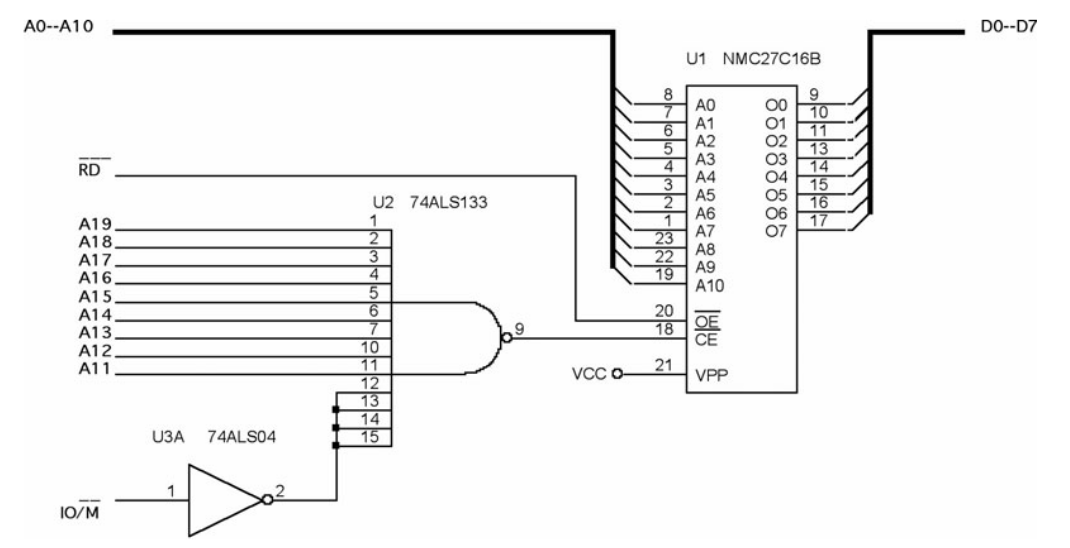
\includegraphics[width = 0.8\textwidth]{./figures/NAND_decoder.png}
  \caption{A simple NAND gate decoder that selects a 2716 EPROM for memory location FF800H–FFFFFH}
  \label{}
\end{figure}
\begin{itemize}
  \item Here, the 2K EPROM is decoded at memory address locations \textbf{FF899H - FFFFFH}.(The FF8 corresponds to 1's in left nine positions)
  \item In such a decoding, one NAND gate decoder selects one 2K EPROM out of many 2K EPROMs that appear in 1M address space.
  \item The obvious disadvantage is that each EPROM needs one NAND gate decoder
\end{itemize}

\subsection{3-to-8 Line Decoder(74LS138)}
\begin{figure}[h!]
  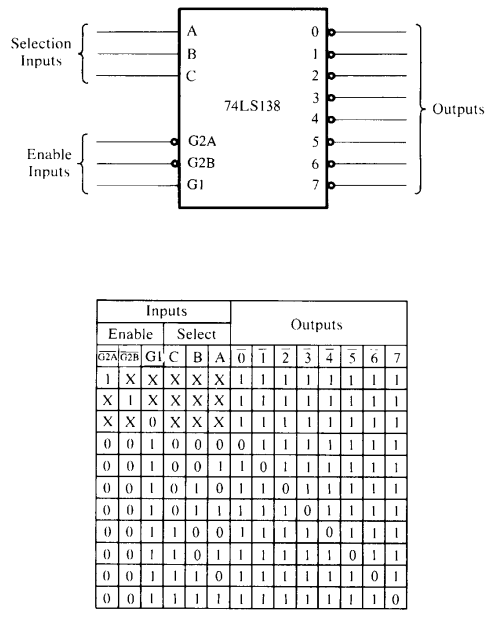
\includegraphics[width = 0.8\textwidth]{./figures/Decoder_3_to_8.png}
  \caption{The 74LS138 3-to-8 line decoder and function table.}
  \label{}
\end{figure}

\begin{itemize}
  \item \textbf{Input}: Enable = 001 and Selection(ABC) = n
  \item \textbf{Input}: $n^{th}output = 0$; all reset are 1
\end{itemize}
\begin{itemize}
  \item \textbf{Input}: $Enable \neq 001$
  \item \textbf{Input}: All outputs are 1
\end{itemize}

\begin{figure}[h!]
  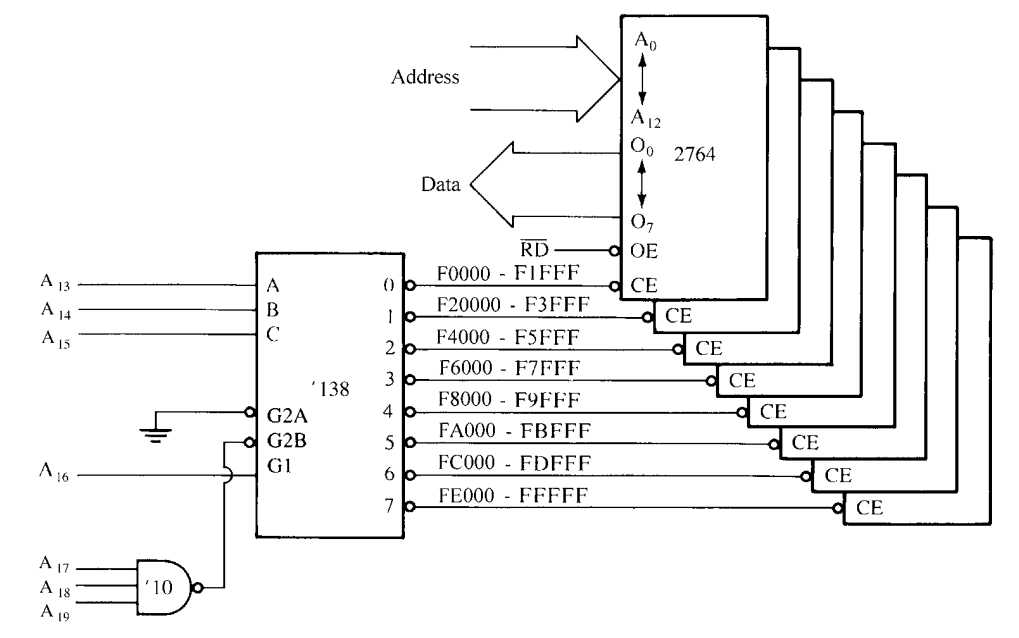
\includegraphics[width = 0.8\textwidth]{./figures/Decoder_Bank.png}
  \caption{A circuit that uses eight 2764 EPROMs for a 64K x 8 section of memory in an
  8088 microprocessor-based system. The addresses selected in this circuit are \textbf{F0000H-FFFFFH}}
  \label{}
\end{figure}
\begin{itemize}
  \item A16-A19 must have 1 for activating 74LS138. Therefore, all addresses begin with "1111" at the left.
  \item Eight 2764 EPROMs (each 8K x 8, having 13 pins) are decoded over address space \textbf{F0000H-FFFFFH}(64K x 8)
\end{itemize}

\section{PROM Address Decoder}
Bipolar PROM is used because of its larger number of input connections, which reduces the number of other circuits required in the decoding system.\newline
\textbf{Example}: 82S147 (512 x 8) PROM has 10 input connections and 8 output connections. Among the input connections, 9 are used for memory addressing (of PROM) with 1 control (G) input. \newline
\begin{figure}[h!]
  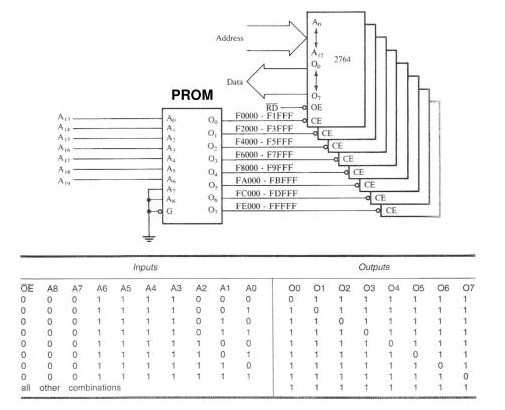
\includegraphics[width = 1.0\textwidth]{./figures/PROM.jpg}
\end{figure}
Here, the control input ($\overline{G}$ or $\overline{CE}$) must be grounded, as if this PROM's outputs float to their high-impedence state, one or more of the PROMs might be selected by noise impulse of the system.
\begin{itemize}
  \item Main advantage of using PROM is that address map can be easily changed.
  \item As the PROM comes with all the locationa programmed as logic 1, only eight of the 512 locations must be programmed.
\end{itemize}

\section{PLD programmable Decoders}
There are three \textbf{Programmable Logic Devices}(PLDs) that function in the same manner:
\begin{enumerate}
  \item PLA (Programmable Logic Array)
  \item PAL (Programmable Array Logic)
  \item GAL (Gated Array Logic)
\end{enumerate}
\begin{itemize}
  \item These devices can be programmed by blowing fumes to establish connections.
  \item The decoding circuit using a PLD is similar as that with a PROM, where the PROM gets replaced by the PLD (programmed with the logic representing the input-output pattern realized by PROM, as shown in a table in the last decoding)
  \item No control or selection logic is required hence. 
\end{itemize}
